\chapter{Somas de variáveis independentes II: Teorema Central do limite}

A pergunta natural depois de ter provado a Lei dos grandes números é a do limite das flutuações da soma $\sum_{k=1}^n X_k$: qual e a boa escala $\varphi(n)$ (com $\lim_{n\to \infty}\phi(n)=\infty$)
para observar um limite não determinístico 
$$\frac{\sum_{k=1}^n X_k - nE[X_i]}{\varphi(n)} \Rightarrow ???.$$
Mas antes de se perguntar a escala o tentar identificar o limite vale a pena de se perguntar em qual sentido pode valer essa convergência.

\medskip

Não podemos obter um limite quase certamente (o em probabilidade). A razão e a seguinte. Como para $k$ fixo 
$(X_1+\dots+X_k)/\varphi(n)$ converge para $0$ e que então o limite seria independente $X_1,\dots, X_k$ para qualquer $k$.
Pela lei do $\{0,1\}$ isso implica que se tiver convergência quase certamente o limite e constante.

\medskip

Mas na verdade o que queremos saber, não e do limite de $\frac{\sum_{k=1}^n X_k - nE[X_i]}{\varphi(n)}$ mas o limite da distribuição da váriavel.
Vamos então introduzir uma noção de convergência adaptada a esse problema.


\section{Convergência fraca}

Em muitos casos é importante termos bem definida uma noção de convergência de medidas de probabilidade.
Supondo por exemplo no espaço mensurável $(E,\mathcal{A})$, tenhamos uma sequência de probabilidades $\mu_n$ e 
gostaríamos de saber se ela converge a uma determinada $\mu$.

Um candidato natural para dara sentido a essa convergência poderia se a distância de variação total entre duas medidas
\begin{equation}
  d_{\VT}(\mu,\nu) = \sup_{A \in \mathcal{A}} |\mu(A) - \nu(A)|.
\end{equation}
Não é difícil mostrar que a definição acima induz uma métrica, mas ela possui alguns problemas que descreveremos a seguir.

\begin{exercise}
  Mostre que $d_{\VT}$ define uma métrica.
\end{exercise}

\begin{exercise}
  Sejam $\mu$ e $\nu$ absolutamente contínuas com respeito a uma medida fixa $\eta$, tendo densidades $\rho$ e $\pi$ respectivamente.
  Encontre uma fórmula para $d_{\VT}(\mu, \nu)$ em termos das densidades.
  Essa fórmula nos remete a qual distância entre funções?
\end{exercise}

Digamos que o espaço amostral $E$ já seja provido de uma métrica $d$ e $\mathcal{A}$ seja a $\sigma$-álgebra dos borelianos em $E$.
Qualquer que seja a noção de convergência que iremos considerar, gostaríamos de dizer que $\delta_{x_n}$ converge a $\delta_x$ sempre que $x_n \to x$ em $E$.
Esse porém não é o caso para $d_{\VT}$, pois se $x_n \neq x$ para todo $n$ e $\{x\} \in \mathcal{A}$, teríamos
\begin{equation}
  d_{\VT}(\delta_{x_n}, \delta_x) \geq |\delta_{x_n}(\{x\}) - \delta_{x}(\{x\}) | = |0 - 1| = 1.
\end{equation}

Aqueles que já viram o conceito de convergência fraca acharão natural que a convergência de $\mu_n$ para $\mu$ seja definida em termos da convergência das integrais $\int f \d \mu_n$ para $\int f \d \mu$.
Porém, como mencionamos no exemplo das medidas $\delta_{x_n}$ acima, gostaríamos também de a convergência respeitasse a topologia original do espaço $E$, o que torna natural o seguinte conceito.

\begin{definition}
  Dizemos que uma sequência de medidas de probabilidade $\mu_n$ converge fracamente (ou converge em distribuição) 
  para uma probabilidade $\mu$ se \index{convergência@convergência!fraca}
  \begin{equation}
    \lim_{n \to \infty} \int f \d \mu_n = \int f \d \mu, \text{ para toda $f:E \to \mathbb{R}$ contínua e limitada.}
  \end{equation}
  Essa convergência muitas vezes é denotada por $\mu_n \Rightarrow \mu$.
\end{definition}

Essa definição fica ainda mais natural para aqueles que conhecem o Teorema da Representação de Riesz.
Com isso em mente, podemos relacionar a convergência em distribuição com a convergência fraca-$\star$ no espaço de medidas finitas.

\begin{exercise}
  Mostre que em $(\mathbb{R}, \mathcal{B}(\mathbb{R}))$, temos que $\tfrac{1}{n} \sum_{i=1}^n \delta_{i/n} \Rightarrow U_{[0,1]}$.
\end{exercise}

\begin{exercise}
  Considere a função $\phi$ do espaço de medidas em $([0,1], \mathcal{B}([0,1]))$ nele mesmo, dada por:
  \begin{equation}
    \phi(\mu)(A) = \tfrac{1}{2} \big( \mu(3A) + \mu(3A - 2) \big).
  \end{equation}
  Identifique o limite em distribuição de $\phi^{(n)}(\delta_0)$.
  Mostre que
  \begin{enumerate}[\quad a)]
  \item a função de distribuição acumulada associada ao limite é contínua,
  \item o limite não é absolutamente contínuo com respeito à medida de Lebesgue.
  \end{enumerate}
\end{exercise}

\begin{exercise}
  Sejam $X_1, X_2, \dots$ i.i.d. distribuidas como $\text{Exp}(1)$ e defina
  \begin{equation}
    M_n = \max_{i = 1, \dots, n} X_i.
  \end{equation}
  Mostre que $M_n - \log(n)$ converge fracamente e identifique o limite.
  Observe que não precisamos dividir $M_n - \log(n)$ por nada para obter a convergência.
\end{exercise}

Nós algumas vezes denotamos $X_n \Rightarrow X$ quando $X_n$ e $X$ são elementos aleatórios de $(\Omega, \mathcal{F}, P)$ 
para descrever a convergência fraca de suas respectivas distribuições. Falamos nesse caso que $(X_n)$ converge para $X$ em distribuição.

\subsection{Um criterio em $\bbR^d$}



Para nos provarmos resultados com convergência fraca, 
e util o resultado seguinte que fala que não precisa verificar convergência para todo $\varphi$ continua limitada. 
Usamos a notação $C^b(\bbR^d)$ e $C^c(\bbR^d)$ pelos espaços de fonções continuas limitadas e continuas com suporte compacto respectivamente

\begin{proposition}\label{prop:dafunca}
As tres seguinte proposições são equivalentes
\begin{itemize}
 \item [(i)] $\forall \varphi \in C^b(\bbR^d), \quad \lim_{n\to \infty} \int_{\bbR^d} \varphi(x)\mu_n(\dd x)= \int_{\bbR^d} \varphi(x)\mu(\dd x).$
 \item [(ii)] $\forall \varphi \in C^c(\bbR^d), \quad \lim_{n\to \infty} \int_{\bbR^d} \varphi(x)\mu_n(\dd x)= \int_{\bbR^d} \varphi(x)\mu(\dd x).$
  \item [(iii)] $\forall \varphi \in H, \quad \lim_{n\to \infty} \int_{\bbR^d} \varphi(x)\mu_n(\dd x)= \int_{\bbR^d} \varphi(x)\mu(\dd x),$\\
  onde $H$ e um subcojunto denso de $C^c(\bbR^d)$ (pela norma de convergência uniforme).
\end{itemize}

\end{proposition}

\begin{proof}
 As implicações  $(i)\Rightarrow (ii) \Rightarrow (iii)$ sendo obvia, sò vamos precisar mostrar $(iii)\Rightarrow (ii)$ e $(ii)\Rightarrow (i)$.
 
Pela primeira implicação, sendo $\gep$, e $\varphi \in C^c(\bbR^d)$ podemos achar $\varphi_{\gep}\in H$ tal que $\|\varphi-\varphi_{\gep} \|\le \gep$.
 Pois temos 
 \begin{multline}
  \limsup_{n\to \infty} |\int \varphi \dd \mu_n-\int \varphi \dd \mu|\\
  \le \limsup |\int (\varphi-\varphi_{\gep}) \dd \mu_n|+|\int \varphi_{\gep} \dd \mu_n-\int \varphi_{\gep}\dd \mu|
  + |\int (\varphi-\varphi_{\gep})\dd \mu|\le 
  2\gep.
 \end{multline}
O que permite a conclusão como $\gep$ e arbitrario.

\medskip

Para $(ii)\Rightarrow (i)$, seja $(f_k)_{k\ge 0}$ una sequencia de funçoes em $C^c(\bbR^d)$ tal que 
$f_k\in [0.1]$, $f_k \uparrow 1$ quando $k \to \infty$. Dado $\varphi \in C^b(\bbR^d)$ definimos $\varphi_k=f_k\varphi \in C^c(\bbR^d)$.
e então por hypotese
$$\lim_{n\to \infty} \int \varphi_k \dd \mu_n= \int \varphi_k \dd \mu  $$ 
Temos 
\begin{equation}
 \begin{split}
 \left |\int (\varphi-\varphi_k) \dd \mu_n \right| & \le  \| \varphi \| \left(1- \int f_k \dd \mu_n \right),\\
    \left|\int (\varphi-\varphi_k) \dd \mu\right| & \le  \| \varphi \| \left(1- \int f_k \dd \mu \right)
 \end{split}
\end{equation}
Então temos 
\begin{multline}
 \limsup_{n\to \infty} \left|\int \varphi\dd \mu_n-\int \varphi\dd \mu_n\right|\\
 \le   \| \varphi \| \left( \limsup_{n\to \infty} \left(1- \int f_k \dd \mu_n \right)
 + \left(1- \int f_k \dd \mu \right) \right) = 2 \| \varphi \| \left(1- \int f_k \dd \mu \right),
\end{multline}
mas o ultimo termo pode ser arbitrariamente pequeno se mandamos $k\to \infty$.
\end{proof}

\subsection{Um criterio em $\bbR$}

\begin{proposition}\label{prop:dafuncao}
Seja $(\mu_n)_{n\ge 0}$ uma sequência de probabilidade em $\bbR$ e $F_n$ as funções acumuladas de distribuição associadas.
Então $\mu_n$ converge fracamente para $\mu$ com  função acumulada de distribuição $F$ se e só se
\begin{equation}\label{eq:acumulex}
 \lim_{n\to \infty} F_n(x):= F(x).
\end{equation}

para todo $x\in \bbR$ onde $F$ é continua (para todo $x$ tal que $\mu(\{x\})=0$.
\end{proposition}


\begin{proof}
Vamos começar mostrando que \eqref{eq:acumulex} implica convergência fraca.
Usando Proposição \ref{prop:dafunca}, e suficiente mostrar $\int f(x) \mu_n(\dd x)$ converge para $f$ diferenciável com suporte compacto.
Lembramos (Proposição \ref{p:espera_acumulada}) que temos 
 $$\int f(x) \mu_n(\dd x)= \int f'(x) (1-F_n(x)) \dd x.$$
 Como $f'$ e limitada e dado que $F(x)$ e descontinua só em conjunto de medida $0$, podemos concluir por convergência dominada que  

 $$\lim_{n\to \infty} \int f'(x) (1-F_n(x)) \dd x=\int f'(x) (1-F_n(x)) \dd x=\int f(x) \mu(\dd x).$$
 
Reciprocamente, se $\mu_n$ converge fracamente para $\mu$, consideramos $x$ um ponto de continuidade de $F$, $\gep>0$ e
$\delta$ tal que 
$$F(x)-(\gep/2) \le F(x-\delta) \le F(x+\delta)\le F(x)+(\gep/2).$$

Consideramos as funções
\begin{equation}
 g^+(u):=\begin{cases}
          1 &\text{ if } u\le x,\\
          1-\delta^{-1}(u-x) \quad &\text{ if } u\in [x,x+\delta],\\
          0 &\text{ if } u \ge x+\delta].
         \end{cases}
\end{equation}
e $g^-(u)=g^{+}(u+\delta)$. Como $\ind_{\{u\le x\}} \le  g^+(u) \le  \ind_{\{u\le x+\delta\}},$
temos 
\begin{equation*}
F_n(x)\le \int g^{+}(u) \mu_n(\dd x)\le \int g^{+}(u) \mu(\dd x)+(\gep/2) \le F(x+\delta)+\gep/2\le F(x)+\gep,
\end{equation*}
 onde a segunda desigualdade pode se deduzir da convergência fraca e vale para $n$ grande suficiente.
Usando $g^-$ podemos provar do mesmo jeito que $F_n(u)\ge F(x)-\gep$, o que acaba a demostração $\gep$ sendo arbitrário. 
 
\end{proof}


\newpage

\begin{topics}
 \section{Tópico : Convergência das medidas empíricas em $\bbR^d$}


Dados $X_1(\go),\dots, X_n(\go)$ uma realização de $n$ variáveis identicamente distribuidas com probabilidade $\mu$, queremos identificar $\mu$.

\medskip

Para isso construímos a medida empírica associada a $X_n$ definida como
\begin{equation}
\mu_{n,\omega}(A):=\frac{1}{n}\sum_{i=1}^n \1_{\{X_i\in A\}}.
\end{equation}
De jeito imediato se $\mu$ for absolutamente continua com respeito a Lebesgue $\mu_{n,\omega}$ e singular com respeito a $\mu$.
Mas os resultado seguinte indica que quando $n\to \infty$, $\mu$ e bem aproximado por $\mu_{n,\omega}$ no sentido da convergência fraca.

\begin{theorem}
 Seja $(X_n)_{n\ge 1}$ uma sequencia de variáveis IID de distribuição $\mu$.
 Então quase certamente temos
 \begin{equation*}
   \mu_{n,\go} \ \Longrightarrow \mu.
 \end{equation*}

 
 
\end{theorem}


\begin{proof}
Seja $H$ um conjunto denso enumerável de $C^c(\bbR^d)$.
Temos que verificar que para todo $\varphi\in H$ 
\begin{equation}
\lim_{n\to \infty} \int \varphi \dd \mu_{n,\go}=  \int \varphi \dd \mu.
\end{equation}
O primeiro termo acima vale 
$$\frac{1}{n}\sum_{i=1}^n \phi(X_i)$$
que converge com probabilidade $1$ para $E[\varphi(X_1)]= \int \varphi \dd \mu.$
Como $H$ e enumerável, a convergência e simultânea para todos $\phi\in H$ com probabilidade $1$,
o que conclui a prova do resultado.

 
\end{proof}







\end{topics}

\newpage

\section*{Intermezzo: a distribuição normal}



Até o presente momento, já sabemos por exemplo que médias empiricas de variáveis aleatórias \iid, 
suficientemente regulares convergem para sua esperança quase certamente.
Vamos fazer contudo um experimento para visualizar esse fenômeno.

Nesse experimento, jogamos $100$ moedas e contamos quantas caras obtivemos.
Pelo que discutimos anteriormente, esperamos que esse número se encontre por volta de $50$, que é a esperança desta soma de variáveis \iid.
Vamos portanto repetir esse experimento mil vezes e observar quantas vezes obtemos algo próximo de $50$, veja Figura~\ref{f:histograma_normal}.

\begin{figure}[!ht]
  \centering
  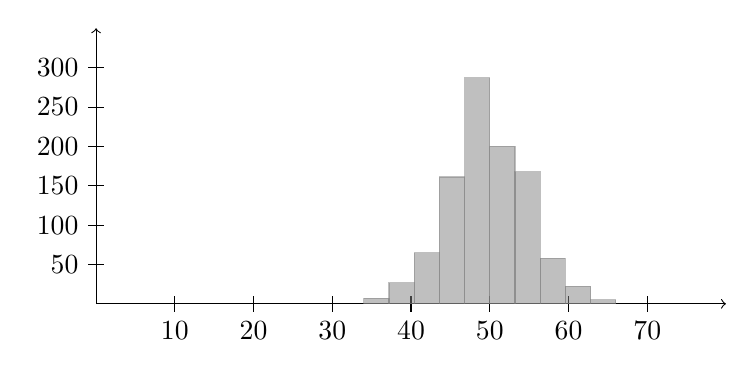
\begin{tikzpicture}[scale=1]
    \draw[<->] (0, 3.5) -- (0,0) -- (8, 0);
    \foreach \x in {10, 20, 30, 40, 50, 60, 70}
    { \draw (.1*\x, -.1) -- (.1*\x, .1);
      \node[below] at (.1*\x, -.1) {$\x$};}
    \foreach \x in {50, 100, 150, 200, 250, 300}
    { \draw (-.1, .01*\x) -- (.1, .01*\x);
      \node[left] at (-.1, .01*\x) {$\x$};}
    \draw[fill, color=gray, opacity=.5] (3.40, 0) rectangle (3.72, 0.07);
    \draw[fill, color=gray, opacity=.5] (3.72, 0) rectangle (4.04, 0.27);
    \draw[fill, color=gray, opacity=.5] (4.04, 0) rectangle (4.36, 0.65);
    \draw[fill, color=gray, opacity=.5] (4.36, 0) rectangle (4.68, 1.61);
    \draw[fill, color=gray, opacity=.5] (4.68, 0) rectangle (5.00, 2.87);
    \draw[fill, color=gray, opacity=.5] (5.00, 0) rectangle (5.32, 2.00);
    \draw[fill, color=gray, opacity=.5] (5.32, 0) rectangle (5.64, 1.68);
    \draw[fill, color=gray, opacity=.5] (5.64, 0) rectangle (5.96, 0.58);
    \draw[fill, color=gray, opacity=.5] (5.96, 0) rectangle (6.28, 0.22);
    \draw[fill, color=gray, opacity=.5] (6.28, 0) rectangle (6.6, 0.05);
  \end{tikzpicture}
  \caption{Vários ensaios de uma variável $\Bin(100,0.5)$, pra ser mais preciso $1000$ ensaios. Cada barra representa o número de ensaios que caíram no intervalo determinado pela base da barra. Note que apesar dos experimentos se concentrarem em torno da média, alguns se afastam um pouco (obviamente pois o experimento é aleatório). Nessa seção estudaremos esses desvios espontâneos, que são chamados de flutuaçãoes. \index{flutuacoes@flutuações}}
  \label{f:histograma_normal}
\end{figure}

Nosso objetivo nessa seção será obter qual é o tamanho típico das flutuações em torno da média dessa soma de variáveis aleatórias.
Ao contrário do que fizemos ao estudar Grandes Desvios, nós agora estamos buscando flutuações menores, 
que acontecem espontaneamente e não com baixa probabilidade.
Note também que apesar de observarmos uma aleatóriedade na Figura~\ref{f:histograma_normal}, 
também notamos uma certa regularidade que muitas vezes é chamada de 'forma de sino' no histograma apresentado.


Começaremos estudando qual poderia ser uma possível forma limite para o histograma da Figura~\ref{f:histograma_normal}.

Como uma primeira tentativa, suponha que $\sum_{i=1}^\infty Z_i$ possui uma certa distribuição $\mu$ (veremos posteriormente que isso somente pode acontecer em casos triviais).
Mas se esse fosse o caso, poderíamos dividir a soma nos termos pares e ímpares $X = \sum_{i \text{ par}} Z_i$ e $Y = \sum_{i \text{ ímpar}} Z_i$.
Nesse caso teríamos $X$ e $Y$ independentes e também distribuídos como $\mu$ (pois são dados por uma soma que tem a mesma distribuição daquela que define $\mu$).

O seguinte lema mostra que isso somente pode acontecer na situação trivial em que $\mu = \delta_0$.

\begin{lemma}
  Sejam $X$ e $Y$ variáveis aleatórias em $\mathcal{L}^2$, \iid com distribuição $\mu$.
  Nesse caso, se $X + Y$ também tem distribuição $\mu$, então $\mu = \delta_0$.
\end{lemma}

\begin{proof}
  Sabemos que
  \begin{equation}
    \begin{split}
      E(X + Y) & = E(X) + E(Y) = 2 E(X) \text{ e}\\
      \Var(X + Y) & = \Var(X) + \Var(Y) = 2 \Var(X).
    \end{split}
  \end{equation}
  Mas como $X + Y$ tem a mesma distribuição de $X$, então $E(X) = 2 E(X)$ e $\Var(X) = 2 \Var(X)$, donde ambas são zero.
  Usando o método dos segundo momento, para todo $a > 0$,
  \begin{equation}
    P[|X| \geq a] \leq \frac{\Var(X)}{a^2} = 0,
  \end{equation}
  terminando a prova de que $X = 0$ quase certamente.
\end{proof}

A intuição dessa prova é que quando somamos duas variáveis não determinísticas, a incerteza da soma (medida atravéz da variância) tende a aumentar.
Dessa forma não podemos obter a mesma distribuição após a soma.

Mas existe uma maneira simples de tornar esse problema interessante novamente.
Digamos que $X$ e $Y$ pertencem a $\mathcal{L}^2$ e são i.i.d.
Então
\begin{equation}
  \Var\Big(\frac{X + Y}{\sqrt{2}}\Big) = 2 \Var\Big( \frac X{\sqrt{2}} \Big) = \Var(X).
\end{equation}
Então podemos nos perguntar se

\begin{question}
  \label{q:ponto_fixo_soma}
  Existe alguma distribuição não trivial $\mu$ em $\mathcal{L}^2$ tal que, se $X$ e $Y$ são independentes e distribuídas de acordo com $\mu$, temos
  \begin{equation}
    \frac{X + Y}{\sqrt{2}} \distr \mu \; ?
  \end{equation}
  Pelo menos sabemos agora que a variância não se altera atravéz dessa operação.
\end{question}

Ou em outras palavras, queremos saber se existe algum ponto fixo para o operador $\Gamma$ que toma uma distribuição $\mu$ em $\mathbb{R}$ e retorna
\begin{equation}
  \label{e:Gamma_operador}
  \Gamma(\mu) = \Big( \frac{X_1 + X_2}{\sqrt{2}} \Big)_* \mu \otimes \mu.
\end{equation}


Para tentar responder a essa questão, vamos estudar mais a fundo qual é a distribuição da soma de duas variáveis aleatórias independentes.
Para isso, considere a distribuição $P_{(X,Y)}$ do par, que coincide com $\mu \otimes \mu$, nos dando
\begin{equation}
  P\Big[ \frac{X + Y}{\sqrt{2}} \leq z \Big] = \mu \otimes \mu \big( \big\{(x, y) \ : \  \tfrac{x + y}{\sqrt{2}} \leq z \big\} \big).
\end{equation}

Note também que a transformação linear $(x,y) \mapsto \tfrac{1}{\sqrt{2}}\big(x + y, x - y\big)$ é uma rotação rígida em $\mathbb{R}^2$, o que nos motiva a propor a pergunta mais simples.

\begin{question}
  Existe alguma distribuição não trivial $\mu$ em $\mathcal{L}^2$ tal que, se $X$ e $Y$ são independentes e distribuídas de acordo com $\mu$, a distribuição do par $(X,Y)$ é invariante por rotações?
\end{question}

Ainda estamos numa busca não rigorosa de tal distribuição, então vamos supor algumas outras propriedades, como por exemplo que $\mu$ seja absolutamente contínua com respeito a Lebesgue, isto é $\d \mu = f(x) \d x$.
Nesse caso, já vimos que $(X, Y) \distr f(x) f(y) \d x \d y$ e no fundo estamos procurando uma função $f$ tal que
\begin{equation}
  f(x) f(y) = h(x^2 + y^2), \text{ para todo $x, y \in \mathbb{R}$ e alguma $h: \mathbb{R}_+ \to \mathbb{R}_+$.}
\end{equation}
Para trasformar o produto $f(x) f(y)$ em uma soma, definimos $g = \log f$ e $k = \log h$ e o que gostaríamos que acontecesse é $g(x) + g(y) = k(x^2 + y^2)$.
Como ainda não estamos preocupados com unicidade de $\mu$ e apenas com a existência, já podemos encontrar nossa resposta para nossa pergunta, escolhendo uma função quadrática, tal como $g(x) = \alpha x^2 - \beta$.

Mas temos ainda que cuidar para que $f(x) = \ex{\alpha x^2 - \beta}$ seja uma densidade, ou seja $\int f \d x = 1$.
Para isso, precisamos que $\alpha$ seja negativo e, fixado $\alpha$, o valor de $\beta$ já estará determinado por normalização.
Tudo isso motiva finalmente a seguinte definição.

\begin{definition}
  Dizemos que $X$ tem distribuição normal canônica, se \index{distribuicao@distribuição!normal}
  \begin{equation}
    \label{e:normal_canonica}
    X \distr \frac{1}{\sqrt{2 \pi}} \exp \big\{-x^2/2\big\} \d x.
  \end{equation}
  Além disso, para $m \in \mathbb{R}$ e $\sigma \geq 0$, dizemos que $Y \distr \mathcal{N}(m, \sigma^2)$ se $Y$ tem a mesma distribuição de $\sigma X + m$, onde $X$ tem distribuição normal canônica $\mathcal{N}(0, 1)$. Note que $\mathcal{N}(m, 0) = \delta_m$.
  Muitas vezes chamamos essa distribuição de gaussiana, obviamente em homenagem a Gauss.
\end{definition}


Vamos rapidamente observar que a definição acima realmente descreve uma distribuição de probabilidade, ou seja que a integral dessa densidade é um.
Para tanto, vamos usar um truque conhecido, que consiste em retornar ao plano.
Obviamente,
\begin{equation}
  \begin{split}
    \Big(\int \exp \big\{-x^2/2\big\} \d x\Big)^2 & = \int \int \exp \big\{-(x^2 + y^2)/2\big\} \d x \d y\\
    & = \int_0^{2 \pi} \int_0^\infty \exp \{ - r^2 / 2 \} r \d r \d \theta \overset{2 s \; = \; r^2}= 2 \pi.
  \end{split}
\end{equation}
Donde a constante em \eqref{e:normal_canonica} está de fato correta.

\begin{exercise}
  Mostre que a distribuição $\mathcal{N}(m, \sigma^2)$, tem densidade
  \begin{equation}
    \frac{1}{\sigma \sqrt{2 \pi}} \ex{-(x - m)^2/(2 \sigma^2)}.
  \end{equation}
\end{exercise}

\begin{exercise}
  Mostre que $Y \distr \mathcal{N}(m, \sigma^2)$ tem esperança $m$ e variância $\sigma^2$.
\end{exercise}

Para confirmar que de fato as distribuições normais se comportam bem com respeito a somas independentes, apresentamos o seguinte resultado.

\begin{proposition}
  \label{p:soma_normais}
  Se $X \distr \mathcal{N}(m, \sigma^2)$ e $Y \distr \mathcal{N}(\bar{m}, \bar{\sigma}^2)$ são independentes, então $X + Y$ tem distribuição $\mathcal{N}(m + \bar{m}, \sigma^2 + \bar{\sigma}^2)$.
  Em particular, $\mu$ é um ponto fixo do operador $\Gamma$ definido em \eqref{e:Gamma_operador}.
\end{proposition}

\begin{proof}
  O caso em que $\sigma$ ou $\bar{\sigma}$ se anulam é trivial, portanto vamos considerar que ambas são positivas.
  Não é difícil ver que podemos também supor que $m = \bar{m} = 0$.
  Podemos então calcular
  \begin{equation}
    P[X + Y \leq a] = P[\sigma W + \bar{\sigma} Z \leq a],
  \end{equation}
  onde $W$ e $Z$ são independentes com distribuição $\mathcal{N}(0,1)$.
  Assim, a probabilidade acima pode ser escrita como
  \begin{equation}
    \label{e:soma_normal}
    \mathcal{N}(0,1) \otimes \mathcal{N}(0,1) \Big( \big\{ (w,z) \in \mathbb{R}^2; \sigma w + \bar{\sigma} z \leq a \big\} \Big).
  \end{equation}
  Agora aplicaremos a rotação rígida $A: \mathbb{R}^2 \to \mathbb{R}^2$ dada por
  \begin{equation}
    A(w,z) = \frac{1}{\sqrt{\sigma^2 + \bar{\sigma}^2}} \big( \sigma w + \bar{\sigma} z, \bar{\sigma} w - \sigma z \big).
  \end{equation}

  Como sabemos que a densidade $f$ de $(W,Z)$ é invariante por $A$, ou seja $f \circ A = f$, então podemos escrever \eqref{e:soma_normal} como
  \begin{equation*}
    \begin{split}
      \mathcal{N}(0,1) & \otimes \mathcal{N}(0,1) \Big( A \big(\big\{ (w,z) \in \mathbb{R}^2; \sigma w + \bar{\sigma} z \leq a \big\} \big) \Big)\\
      & = \mathcal{N}(0,1) \otimes \mathcal{N}(0,1) \Big( \Big\{(w,z); \frac{1}{\sqrt{\sigma^2 + \bar{\sigma}^2}}w \leq a \Big\} \Big)\\
      & = \mathcal{N}(0,1) \big( (-\infty, a \sqrt{\sigma^2 + \bar{\sigma}^2} \big] \big) = \mathcal{N}(0,\sigma^2 + \bar{\sigma}^2) \big( (-\infty, a \big] \big),
    \end{split}
  \end{equation*}
  terminando a prova da proposição.
\end{proof}

Podemos obter um corolário interessante sobre a soma de normais i.i.d.
\begin{corollary}
  \label{c:normaliz_normais}
  Sejam $X_1, X_2, \dots$ variáveis \iid com distribuição $\mathcal{N}(m,\sigma^2)$, então
  \begin{equation}
    X_1 + \dots + X_n \distr \mathcal{N}(nm, n \sigma^2).
  \end{equation}
  Como consequência
  \begin{equation}
    \frac{\sum_{i=1}^n X_i - n E(X_1)}{\sigma \sqrt{n}} \distr \mathcal{N}(0,1).
  \end{equation}
\end{corollary}

Lembrando da Lei dos Grandes Números, se dividimos a soma dos $X_i - E(X_i)$ por $n$, essa fração vai a zero quase certamente.
O que concluímos acima é que ao dividir por $\sqrt{n}$ obtemos um limite não trivial (nem zero, nem infinito) e aleatório (não determinístico).

Mais uma observação curiosa: nossa motivação para a definição da distribuição normal passou por invariância por rotações e podemos extender essa invariância para $n$ normais independentes.
Note que somar as coordenadas canônicas é equivalente a tomar o produdo escalar com o vetor $(1,1,\dots,1)$, que tem norma euclideana $\sqrt{n}$.

Uma outra maneira de entender o corolário acima é que a normal é um ponto fixo da operação seguinte
\begin{enumerate}[\quad a)]
\item tome uma distribuição $\mu \in \mathcal{L}^2$,
\item considere $X_1, \dots, X_n$ \iid com distribuição $\mu$ e
\item retorne a distribuição de
  \begin{equation}
    \frac{X_1 + \dots + X_n - n E(X_1)}{\sqrt{n}}.
  \end{equation}
\end{enumerate}

Na Questão~\ref{q:ponto_fixo_soma}, nos perguntamos quais seriam os outros possíveis pontos fixos de $\Gamma$ e isso será considerado depois.
Mas uma outra questão bastante importante é se o ponto fixo $\mathcal{N}(0,1)$ é atrator, ou seja se começando com outras distribuições poderíamos nos aproximar de $\mathcal{N}(0,1)$ à medida que iteramos $\Gamma$.

Isso é estudado no Teorema Central do Limite (TCL) que provaremos posteriormente.
Mas antes, precisamos desenvolver uma boa definição de convergência para distribuições, ou em outras palavras definir uma topologia.
Esse será o nosso próximo tópico.



\section{Funções características}

Esta seção trata da função característica de uma variável aleatória, que pode ser vista como um análogo complexo da trasformada de Laplace, ou também como a transformada de Fourier de uma distribuição em $\mathbb{R}$.
   Vamos estudar suas principais propriedades e demonstrar que a função características determinam unicamente a distribuição da variável aleatória.
 
   \begin{definition}
Dada uma variável aleatória $X$, a função característica de $X$, $\widebar{\phi}_{X}:\mathbb{R^d} \rightarrow \mathbb{C}$, é definida por
     \begin{equation}
      \hat{\phi}_{X}(\xi):=E[e^{i \xi.X}], \qquad \forall \xi \in \mathbb{R^d}.
     \end{equation}
     onde $.$ denote o produto scalar usual.
     
     
  \end{definition}

Essa função caracteristica pode tambem ser interpretada com a transformade de Fourier da distribuição de $P_X$ (que escrevemos $\hat P_X$), definida por 
$$ \hat \mu(\xi):=\int_{\bbR^d}e^{i \xi.x} \mu(\d x)$$
O teorema de convergência dominada garante que $\hat{\phi}_{X}$ e continua.


\medskip

   \begin{lemma}
Seja $X$ uma variável gaussiana de distribuição $\cN(0,\sigma)$,
então temos 
\begin{equation}
   \hat{\phi}_{X}(\xi):= e^{- \frac{\sigma^2 \xi^2}{2}}.
\end{equation}

  \end{lemma}
  \begin{proof}
  Temos 
  \begin{equation}
   \hat{\phi}_{X}(\xi):=\frac{1}{\sigma \sqrt{2\pi}}\int_{\bbR} e^{-\frac{x^2}{2\sigma^2}} e^{i\xi x}\dd x.
  \end{equation}
E suficiente tratar o caso $\sigma=1$, pois os outros casos podem ser obtidos por substitução $x=\sigma y$.
   Por simetría, a parte imaginária da integral vale zero.
   Pois so temos que calcular 
   \begin{equation}
   f(\xi):= \frac{1}{\sqrt{2\pi}}\int_{\bbR} e^{-\frac{x^2}{2}} \cos(\xi x) \dd x.
   \end{equation}
 Derivando a função na integral (o que podemos fazer por que $|x e^{-\frac{x^2}{2}}|$ e integravel) temos
 \begin{equation}
  f'(\xi):=- \frac{1}{\sqrt{2\pi}}\int_{\bbR} e^{-\frac{x^2}{2}} x \sin(\xi x) \dd x.
 \end{equation}
Pois integrando por parte obtemos 
 \begin{equation}
  f'(\xi):=- \frac{1}{\sqrt{2\pi}}\int_{\bbR} e^{-\frac{x^2}{2}} \xi \cos(\xi x) \dd x= -\xi f(\xi).
 \end{equation}
   Então $f$ e solução da equação diferential $f'(\xi)+ \xi f(\xi)=0$, o que, junto com a condição $f(0)=0$
   da o resultado $f(\xi)= \exp(-\xi^2/2)$.
  \end{proof}


  \begin{theorem}
   A função característica $\hat \phi_X$ determina a distribuição de $X$, o de jeito equivalente, 
   a transformação $\mu \to \hat \mu$ e injectiva (no espaço das probabilidade em $\bbR^d$).
  \end{theorem}

  \begin{proof}
   Consideramos o caso $d=1$ primeiro. Chamamos $g_{\sigma}$ a densidade da lei gaussiana 
   $$ g_{\sigma}(x):=\frac{1}{\sigma \sqrt{2\pi}} e^{-\frac{x^2}{2\sigma^2}}, \qquad x \in \bbR.$$ 
   Definimos $\mu_{\sigma}$ a convolução de $\mu$ com $g_{\sigma}$ do jeito seguinte 
   \begin{equation}
   \begin{split}
 f_{\sigma}(x)&:= \int_{\bbR} g_{\sigma}(x-y)\mu(\dd y)= g_{\sigma}\ast\mu,\\    
 \mu_{\sigma}(x)&:= f_{\sigma}(x) \dd x.   
   \end{split}
 \end{equation}
Vamos mostrar primeiramente que para todo $\sigma>0$,  $\mu_{\sigma}$ e determinada por $\hat \mu$, e pois mostraremos que para 
toda função $\varphi$ continua limitada
   \begin{equation}\label{covigi}
  \lim_{\sigma \to 0} \int_{\bbR} \varphi(x)\mu_{\sigma}( \dd x):= \int_{\bbR} \varphi(x)\mu( \dd x ).
   \end{equation}
Pelo primeiro ponto vamos usar o lema precedente que nos diz que 
\begin{equation}
 g_{\sigma}(x)= (\sigma \sqrt{2\pi})^{-1} \int_{\bbR} e^{i\xi x} g_{1/\sigma}(\xi) \dd \xi.
\end{equation}
Em consequencia temos como consequencia do teorema de Fubini (verificando integrabilidade)
\begin{equation}\begin{split}
 f_{\sigma}(x)= \int_{\bbR}g_{\sigma}(x-y)\mu(\dd y)&= 
 (\sigma \sqrt{2\pi})^{-1} \int_{\bbR}\left(\int_{\bbR} e^{i\xi(y-x)} g_{1/\sigma}(\xi)  \dd \xi\right) \mu(\dd y) \\
 &= (\sigma \sqrt{2\pi})^{-1} \int_{\bbR} g_{1/\sigma}(\xi) e^{-i\xi x} \left(\int_{\bbR} e^{i\xi y}  \mu(\dd y) \right) \dd \xi \\
 &=(\sigma \sqrt{2\pi})^{-1} \int_{\bbR} g_{1/\sigma}(\xi) e^{-i\xi x} \hat\mu(\xi) \dd \xi.
\end{split}
 \end{equation}
Agora mostramos \eqref{covigi}. Temos, usando Fubini que para $\phi$ continua limitada

\begin{multline}
 \int_{\bbR} \varphi(x)\mu_{\sigma}( \dd x)= \int_{\bbR} \varphi(x) \left(\int_{\bbR} g_\sigma(y-x) \mu(\dd y)\right) \dd x \\
   \int_{\bbR} \left( \int_{\bbR} \varphi(x)  g_\sigma(y-x) \dd x \right) \mu(\dd y)=  \int_{\bbR}  \varphi\ast g_\sigma(y) \mu(\dd y).
 \end{multline}
Pois, usando  
\begin{equation}
 \int_{\bbR} g_\sigma(x) \dd x \quad \text{ and } \quad \forall \gep>0  \, \lim_{\sigma\to 0} \int_{\{ |x|>\gep \}} g_\sigma(x) \dd x=0, 
\end{equation}
e facil mostrar que para todo $y$ 
\begin{equation}
  \lim_{\sigma \to 0} \varphi\ast g_\sigma(y)=\varphi(y).
\end{equation}
Pois concluimos por convergência dominada (lembra que $\phi$ e limitada e $|\varphi\ast g_\sigma(x)|\le \sup |\phi|$) que \eqref{covigi} vale.

\medskip

O caso geral $d\ge 1$ e similar, trocando $g_{\sigma}$ pela seguinte versão multidimensional. 
$$g_{\sigma}^{(d)}(x):=\prod_{i=1}^d g_{\sigma}(x_i).$$
\end{proof}


Acabamos essa introdução a funçoes característica com a observação seguinte

\begin{proposition}\label{prop:taylorcara}
 Sejà $X=(X_1,\dots,X_d)$ um vetor aleatório em $\cL^2(\bbR^d)$ (todas coordenadas possuem segundo momento). Então $\hat \phi_X(\xi)$ e $C^2$ e
 temos na vizinhança de zero
 \begin{equation}\label{taylorblabla}
  \hat \phi_X(\xi)=1+i \sum_{j=1}^d \xi_j E[X_j]- \frac{1}{2} \sum_{j=1}^d\sum_{k=1}^d \xi_j \xi_k E[X_j X_j]+ o(|\xi|^2).
 \end{equation}
\end{proposition}

  \begin{proof}
   Como todos as coordenadas ficam em $\cL^2$ podemos usar teoremas usuais de derivação de integrais  para obter que 
   \begin{equation}
    \frac{\partial  \hat \phi_X}{\partial \xi_i}(\xi)=  iE[X_i e^{\xi.X}] \quad \text{ and }  \frac{\partial^2  \hat \phi_X}{\partial \xi_j \partial \xi_k}(\xi) 
    \hat \phi_X(\xi)=-E[X_jX_k e^{\xi.X}].
   \end{equation}
   que são funçoes continuas por convergência dominada.
O segundo resultado segue da formula de Taylor applicada em zero.
  \end{proof}
Observamos que o resultado acima pode ser extendido no caso $\cL^p$ mas o caso $\cL^2$ e de maior importancia para nosso objetivo. 

% 
% 
% 
% \begin{topics}
% 
%   \section[Tópico: Funções características]{Tópico: Funções características \footnote{Somos gratos a Rangel Baldasso por escrever essa seção.}}
% 
%   Esta seção trata da função característica de uma variável aleatória, que pode ser vista como um análogo complexo da trasformada de Laplace, ou também como a transformada de Fourier de uma distribuição em $\mathbb{R}$.
%   Vamos estudar suas principais propriedades e demonstrar que a função características determinam unicamente a distribuição da variável aleatória.
% 
%   \begin{definition}
%     Dada uma variável aleatória $X$, a função característica de $X$, $\widebar{\phi}_{X}:\mathbb{R} \rightarrow \mathbb{C}$, é definida por
%     \begin{equation}
%       \widebar{\phi}_{X}(t)=\mathbb{E}(e^{itX}), \qquad t \in \mathbb{R}.
%     \end{equation}
%   \end{definition}
% 
%   Vamos começar estudando as propriedades básicas de $\widebar{\phi}_{X}$.
% 
%   \begin{exercise}
%     Prove que a função $\widebar{\phi}_{X}$ é absolutamente contínua.
%   \end{exercise}
% 
%   \begin{exercise}
%     Suponha que $\mathbb{E}(|X|^{n}) < +\infty$. Prove que a função $\widebar{\phi}_{X}$ é $n$ vezes diferenciável em $t=0$ e que $\widebar{\phi}_{X}^{(n)}(0)=i^{n}\mathbb{E}(X^{n})$.
%   \end{exercise}
% 
%   \begin{exercise}
%     Se $X_{1}, X_{2}, \ldots, X_{n}$ são independentes e $a_{1}, a_{2}, \ldots, a_{n} \in \mathbb{R}$, então
%     \begin{equation}
%       \widebar{\phi}_{a_{1}X_{1}+a_{2}X_{2}+\cdots+a_{n}X_{n}}(t)=\widebar{\phi}_{X_{1}}(a_{1}t)\widebar{\phi}_{X_{2}}(a_{2}t)\cdots\widebar{\phi}_{X_{n}}(a_{n}t).
%     \end{equation}
%   \end{exercise}
% 
%   Como vamos ver agora, a função característica nos permite recuperar a distribuição de $X$:
% 
%   \begin{exercise}
%     Use a seguinte igualdade
%     \begin{equation}
%       \lim_{T \rightarrow +\infty}\int_{0}^{T}\frac{\sin(tz)}{t}\,\d t=\begin{cases}
%         (\pi/2) & \text{se } z > 0 \\
%         0 & \text{se } z = 0 \\
%         -(\pi/2) & \text{se } z < 0 \\
%       \end{cases}
%     \end{equation}
%     para provar que se $a<b$ são pontos de continuidade da função de distribuição de $X$, $F_{X}$, então
%     \begin{equation}
%       F_{X}(b)-F_{X}(a)=\lim_{T \rightarrow +\infty} \frac{1}{2\pi}\int_{-T}^{T}\frac{e^{-itb}-e^{-ita}}{-it}\widebar{\phi}_{X}(t)\,dt.
%     \end{equation}
%     Conclua que a distribuição de $X$ é determinada por $\widebar{\phi}_{X}$.
%   \end{exercise}
% 
%   \par O próximo exercício consiste em calcular algumas funções características.
% 
%   \begin{exercise}
%     Calcule as funções características das seguintes distribuições:
%     \begin{itemize}
%     \item[i.] $X \sim Ber(p)$;
%     \item[ii.] $X \sim Poisson(\lambda)$;
%     \item[iii.] $X \sim N(0,1)$. \textit{Dica: fixe $z \in \mathbb{R}$, calcule $\mathbb{E}(e^{zX})$ e use o Princípio da continuação analítica.}
%     \end{itemize}
%   \end{exercise}
% \end{topics}





\section{O Teorema de Levy}

O Teorema de Levy nos leva uma conexão entre a noção de função característica e a convergência fraca.


\begin{theorem}
 Uma sequencia de distribuição $\mu_n$ converge fracamente para $\mu$ se e sò se 
 \begin{equation}
  \forall \xi \in \bbR^d, \quad \lim_{n\to \infty}\hat \mu_n(\xi)=\hat \mu(\xi).
 \end{equation}
\end{theorem}


\begin{proof}
 Uma implicação do teorema segue imediatamente da definição da convergência fraca pois 
 $x \to e^{x.\xi}$ e continua e limitada então 
 \begin{equation}
 \lim_{n\to \infty}\int_{\bbR^d} e^{\xi.x} \mu_n(\dd x)=\int_{\bbR^d} e^{\xi.x} \mu(\dd x).
 \end{equation}

 \medskip
 
 Mostramos agora a recíproca no caso $d=1$ (o caso geral $d\ge 1$ segue de jeito analogo).
 Sendo $f\in C^c(\bbR)$ e $g_{\sigma}$ definido por 
 $$ g_{\sigma}(x)=(\sigma \sqrt{2\pi})^{-1} \exp\left(-\frac{x^2}{2\sigma^2}\right) $$
 reparamos que $f\ast g_{\sigma}$ converge uniformemente por $f$ quando $\sigma \to 0$, pois 
 $f$ sendo absolutamente continua temos
 \begin{multline}
  \left |\int f(x-y) g_{\sigma}(y) \dd x -f(x) \right|\\
  =   |\int (f(x-\sigma y)-f(x)) g_{1}(y) \dd x|
  \le \int \go_f(\sigma |y|) g_{1}(y) \dd x
 \end{multline}
onde $\go_f(t):= \max_{|x-y|\le t} |f(x)-f(y)|$, e podemos concluir por convergência dominada.
Então pela Proposição \ref{prop:dafuncao} vai ser sufficiente de verificar a convergência para 
$$H:= \{ \varphi=f \ast g_{\sigma}\ : \ \sigma>0, \ f\in C^c(\bbR)  \}$$ 
 que fica denso em $C^c(\bbR^d)$.
 
 \medskip
 
 A computação para provar a injectividade da transformada de Fourier, temos para qualquer probabilidade $\nu$
 \begin{multline}
  \int f \ast g_{\sigma} \ \dd \nu= \int f(x) g_{\sigma} \ast \nu(x) \dd x\\
  =\int f(x)  \left( (\sqrt{2\pi} \sigma)^{-1}\int e^{-i\xi x}g_{1/\sigma}(\xi) \hat \nu(\xi) 
  \dd 
  \xi \right) \dd x.
 \end{multline}
Como $\hat \mu_n(\xi) \to \hat \mu(\xi)$, por convergência dominada temos para todo $x$
 $$\int e^{-i\xi x}g_{1/\sigma}(\xi) \hat \mu_n(\xi) 
  \dd 
  \xi  \to \int e^{-i\xi x}g_{1/\sigma}(\xi) \hat \mu(\xi) 
  \dd 
  \xi.$$
  Usando de novo convergência dominada (as integrais são acima são menor que $1$ em valor absoluta) pela integral em $x$, concluimos que 
  \begin{equation}
    \lim_{n\to \infty} \int f \ast g_{\sigma} \dd \nu_n = \int f \ast g_{\sigma} \dd \nu.
  \end{equation}
O que conclui a demostração.
\end{proof}


\section{O teorema central do limite para sequências IID}


\subsection{O teorema central do limite em $\bbR$}

Agora estamos pronto para mostrar 
\begin{theorem}
 Seja $(X_n)_{n\ge 1}$ uma sequencia uma sequencia de variáveis aleatórias em $\cL^2$, de varianca $\sigma^2$.
 Então temos a seguinte convergência em distribuição 
 
 \begin{equation}
  \frac{1}{\sqrt{n}}\left(X_1+\dots+X_n-n E[X_1]\right) \Rightarrow \cN(0,\sigma^2)
 \end{equation}

 De jeito equivalente temos para todos reais $a<b$ 
 
 \begin{equation}
 \lim_{n\to \infty} P\left[  X_1+\dots+X_n\in [nE[X_1]+\sqrt{n}a \ ,\  nE[X_1]+\sqrt{n}b]\right]=\frac{1}{\sigma \sqrt{2\pi}} \int^b_a e^{\frac{x^2}{2\sigma^2}} \dd x.
 \end{equation}

 
\end{theorem}

\begin{proof}
 Pelo teorema de Levy, e sufficiente de mostrar convergência pontual das funçoes caracteristica.
 Nota que podemos se satisfazer da prova quando $E[X_1]=0$ substituindo $X$ por $X-E[X]$ se for necessario.
 Definimos $Z_n:= \frac{1}{\sqrt{n}}\left(X_1+\dots+X_n\right).$
 Temos 
 
 \begin{multline}
  \hat \phi_{Z_n}(\xi)=E\left[\exp\left( \frac{i\xi}{\sqrt{n}}\left(X_1+\dots+X_n\right) \right)  \right]\\=
  E\left[ \exp\left( \frac{i\xi X_1}{\sqrt{n}} \right) \right]^{n}=  \hat \phi_{X_1}(n^{-1/2}\xi)^n.
 \end{multline}
Sabemos da Proposição \ref{prop:taylorcara} que quando $\xi\to 0$
\begin{equation}
 \hat \phi_{X_1}(\xi)= 1-\frac{\xi^2\sigma^2}{2}+o(\xi^2),
\end{equation}
então temos par $\xi$ fixo
\begin{equation}
  \hat \phi_{X_1}(n^{-1/2}\xi)=1- \frac{\xi^2\sigma^2}{2n}+o(n^{-1}),
\end{equation}
e podemos concluir que 
\begin{equation}
 \lim_{n\to \infty} \hat \phi_{X_1}(n^{-1/2}\xi)^n= e^{-\frac{\sigma^2\xi^2}{2}}.
\end{equation}
Como sabemos que essa ultima quantidade e a função caracteristica de $\cN(0,\sigma^2)$ isso acaba a demostração.
 
 \medskip
 
 A formulação equivalente pode ser obtida aproximando $\1_{[a,b]}$ com funções continua (isso funciona por que a distribuição Gaussiana não possui cojuntos unidade tendo probabilidade positiva). 
 
\end{proof}





No caso especial em que $E = \mathbb{R}$, temos vários outras maneiras de caracterizar convergência em distribuição.
A primeira é dada pela seguinte

\begin{proposition}
  \label{p:conv_distr_suave}
  Se $\int g \d \mu_n$ converge para $\int g \d \mu$ para toda $g \in C^3$ limitada e com as três primeiras derivadas limitadas, então $\mu_n \Rightarrow \mu$.
\end{proposition}

\begin{proof}
  Primeiramente, vamos ver que podemos nos concentrar em um conjunto compacto da reta.

  Para isso fixe um $\varepsilon > 0$ e tome $M'$ tal que $\mu\big( [-M', M'] \big) > 1 - \varepsilon / 3$.
  Tomando uma função $g$ satisfazendo as hipóteses do teorema e tal que
  \begin{equation}
    \1{[-M',M']} \leq g \leq \1{[-M'-1,M'+1]},
  \end{equation}
  concluimos que
  \begin{equation}
    \mu_n \big( [-M'-1, M'+1] \big) \geq 1 - \varepsilon/2,
  \end{equation}
  para todo $n$ suficientemente grande.
  Se tomamos $M \geq M'$ suficientemente grande, podemos obter a cota acima para todo $n$ (com $M$ no lugar de $M'+1$ e $\varepsilon$ no lugar de $\varepsilon/2$).

  Fixamos agora uma $f: \mathbb{R} \to \mathbb{R}$ contínua e limitada.
  Sabemos que é possível aproximar $f$ por uma função $g \in C^3$ de suporte compacto, com $\lVert g \rVert_\infty \leq 2 \lVert f \rVert_\infty$ e $|g - f| \leq \varepsilon/M$ uniformemente no intervalo $[-M,M]$.
  Essa $g$ certamente satisfaz as hipóteses do teorema.

  Portanto,
  \begin{equation*}
    \begin{split}
      \Big| \int f \d \mu_n - \int f \d \mu\Big| & \leq 2 \varepsilon \lVert f \rVert_\infty + \Big| \int_{-M}^M f \d \mu_n - \int_{-M}^M f \d \mu\Big|\\
      & \leq 2 \varepsilon \lVert f \rVert_\infty + \frac \varepsilon{M} 2 M + \Big| \int_{-M}^M g \d \mu_n - \int_{-M}^M g \d \mu\Big|\\
      & \leq 2 \varepsilon \lVert f \rVert_\infty + 2 \varepsilon + \Big| \int g \d \mu_n - \int \d \mu\Big|.
    \end{split}
  \end{equation*}
  Como o último termo converge a zero e $\varepsilon$ foi escolhido arbitrariamente, isso conclui a prova da proposição.
\end{proof}


\subsection{O Teorema Central do Limite em $\bbR^d$}

Para formular o teorema central do limite em dimenção superior precisamos introduzir umas noções. 
Se $X=(X^{(1)},\dots,X^{(d)})$ e um veitor aleatório em $\cL^1$. Definimos a esperança de $X$ como seguinte
$$E[X]= (E[X^{(1)}],\dots,E[X^{(d)}]).$$


\begin{definition}
 Uma veitor aleatório $(X^{(1)},\dots X^{(d)})$ e chamado de veito gaussiano, se para qualquer $(\gl_1,\dots,\gl_d)$
 a distribuição de 
 $\gl_1 X^{(1)} +\dots+\gl_d X^{(d)}$.
\end{definition}

\begin{exercise}
 Mostrar que se $X=(X^{(1)},\dots X^{(d)})$ e um veitor gaussiano então $X^{(1)},\dots,X^{(d)}$ são variáveis gaussiana, mas que a reciproca e falsa quando $d\ge 2$. 
\end{exercise}


Fica claro que se para uma sequência de veitores $(X_n)_{n\ge 1}$ IID em $\cL^2$ temos
$$ \frac{1}{\sqrt{n}}( (X_1+\dots+X_n) -nE[X_1])\ \Longrightarrow \ X, $$
o veitor $X$ precisa ser Gaussiano. Para ver isso e sufficiente aplicar o teorema central limite para  
$\gl_1 X^{(1)} +\dots+\gl_d X^d.$

\medskip

Uma segunda observação e que a distribuiçã de um veitor gaussiano e totalmente definida por sua media 
$E[X]$
a sua matrice de covariança
\begin{equation}
 \Sigma_X:=(\sigma_X(i,j))_{i,j=1}^d, \quad  \text{onde} \quad \sigma_X(i,j):= \Cov(X^{(i)}X^{(j)}).
\end{equation}
Para ver isso consideramos o caso $E[X]=0$ (o outro caso sendo similar) 
e sendo $X$ um veitor gaussiano cuja matrice de covariança $\Sigma$ calculamos a função caracteristica.
Por definição, $\xi.X$ sendo uma combinação linear das coordenadas, tem uma distribuição Gaussiana.
Pois temos
\begin{equation}
\Var(\xi.X)=\sum_{i,j=1}^d \sigma(i,j) \xi_i \xi_j= (\xi. \Sigma \xi).
\end{equation}
Então
\begin{equation}
 \hat \phi_X(\xi)= E[e^{i\xi.X}]=\exp\left(-\frac{(\xi. \Sigma \xi)}{2}\right).
\end{equation}

No caso onde $\Sigma$ a a matrice identidade, e facil de ver que o veitor gaussiano correspondente pode ser obtido 
considerando $X^{(1)},\dots,X^{(d)}$ sendo variáveis gaussianas independente de variança $1$. Dai podemos costruir um vector gaussiano para $\Sigma$ arbitrario.


\begin{proposition}
Para toda matrix $\Sigma$ simetrica positiva, existe um veitor gaussiano de matrice de covariança $\Sigma$.  
\end{proposition}
Em geral escrevemos $\cN(m,\Sigma)$ pela distribuição do veito gaussiano de matrice de covariança $\Sigma$ e de media (esperança) $m\in \bbR^d$.

\begin{proof}
 Seja $M$ a matrice simetrica positiva tal que $M^2=\Sigma$ ($M=\sqrt{\Sigma}$), e $Z$ um veitor gaussiano de distribuição $\cN(m,\Sigma)$.
 Definimos $X=MZ$ e verificamos que 
 \begin{equation}
 E[X^{(i)}X^{(j)}]=E[ \left(\sum_{k=1}^d m_{i,k} Z^{(k)}\right)\left(\sum_{k=1}^d m_{j,k} Z^{(k)}\right)]= \sum_{k=1}^d m_{i,k}m_{j,k}= \sigma(i,j).
\end{equation} 
 \end{proof}


\begin{theorem}
 Seja $(X_n)_{n\ge 1}$ uma sequencia de veitores aleatóries em $\cL^2$, de matriz de covarianca $\Sigma$.
 Então temos a seguinte convergência em distribuição 
 
 \begin{equation}
  \frac{1}{\sqrt{n}}\left(X_1+\dots+X_n-n E[X_1]\right) \Rightarrow \cN(0.\Sigma).
 \end{equation}

\end{theorem}

Deixamos a demostração como exercicio jà que e identica ao caso $d=1$.



\newpage

\subsection{O TCL para uma sequência i.i.d.}

\begin{theorem}[Teorema Central do Limite]
  \index{Teorema!Central do Limite}
  \label{t:tcl_iid}
  Considere em $(\Omega, \mathcal{F}, P)$, uma sequência $X_1, X_2, \dots$ de variáveis aleatórias \iid em $\mathcal{L}^3$.
  Nesse caso, se definimos $m = E(X_1)$ e $\sigma^2 = \Var(X_1)$, temos
  \begin{equation}
    \frac{\sum_{i=1}^n (X_i - m)}{\sigma \sqrt{n}} \Rightarrow \mathcal{N}(0,1).
  \end{equation}
\end{theorem}

\begin{proof}
  Primeiramente, observe que podemos supor que $m = 0$, pois de qualquer forma iremos subtrair a média da distribuição na qual nos interessamos.
  Uma outra observação importante é que podemos supor $\sigma = 1$, pois no caso geral de qualquer forma estamos somando $X_i/\sigma$ no enunciado.

  Como vimos na Proposição~\ref{p:conv_distr_suave}, basta mostrar a convergência das integrais de funções $g \in C^3$, que possuam todas as três primeiras derivadas limitadas.
  Considerando a função
  \begin{equation}
    \phi^n(x_1, \dots, x_n) := g\Big(\frac{x_1 + \dots + x_n}{\sqrt{n}} \Big),
  \end{equation}
  nos basta provar a convergência das sequências de números reais
  \begin{equation}
    \label{e:tcl_limite_phi}
    \lim_n \int \phi^n(X_1, \dots, X_n) \d P = \int g(s) \mathcal{N}(0,1)(\d s).
  \end{equation}

  Vale lembrar que no Corolário~\ref{c:normaliz_normais} já estabelecemos algo mais forte para variáveis normais.
  Mais precisamente, suponha que extendemos nosso espaço de probabilidade para $(\Omega', \mathcal{F}', P')$, onde exista uma sequência $Y_1, Y_2, \dots$ de variáveis aleatórias \iid com distribuição $\mathcal{N}(0,1)$ independente de $X_1, X_2, \dots$
  Então, para todo $n \geq 1$,
  \begin{equation}
    \int \phi^n(Y_1, \dots, Y_n) \d P' = \int g(s) \mathcal{N}(0,1) (\d s),
  \end{equation}
  o que tornaria o limite em \eqref{e:tcl_limite_phi} trivial para tais variáveis.
  A nossa estratégia será aproximar $\phi^n(X_1, \dots, X_n)$ por $\phi(Y_1, \dots, Y_n)$, e faremos isso trocando uma variável de cada vez.

  Para entender o que acontece quando trocamos uma das variáveis $X_i$ por $Y_i$, temos que expandir $g$ em série de potências, isto é, escrever
  \begin{equation}
    g(s) = g(s_0) + g'(s_0)(s - s_0) + g''(s_o)(s-s_0)^2/2 + r_{s_0}(s - s_0),
  \end{equation}
  onde $r_{s_0}(h)/h^3$ é limitada por $M$, uniformemente em $h$ e $s_0$ em consequência das nossas suposições sobre $g$.

  Denotando $z_i = (y_1, \dots, y_{i-1}, x_i, \dots x_n)$, $z_i^o := (y_1, \dots, y_{n-1}, 0, x_{n+1}, \dots, x_n)$ e $s_i^o = y_1 + \dots + y_{n-1} + x_{n+1} + \dots x_n$, temos
  \begin{equation}
    \phi^n(z_i) %& = \phi^n(z_i^o) + \frac{\partial \phi^n}{\partial x_i} (z_i^o) x_i + \frac{\partial^2 \phi^n}{\partial x_i^2} (z_i^o) \frac{x_i^2}{2} + r_z(x_i)\\
    = \phi^n(z_i^o) + g' \Big( \frac{s_i^o}{\sqrt{n}} \Big) \frac{x_i}{\sqrt{n}} + g'' \Big( \frac{s_i^o}{\sqrt{n}} \Big) \frac{x_i^2}{2n} + r_{\frac{s_i^o}{\sqrt{n}}} \Big( \frac{x_i}{\sqrt{n}} \Big),
  \end{equation}
  Nós propositalmente expandimos $\phi^n$ até ordem dois, pois $X_i$ e $Y_i$ possuem os mesmos momentos de ordem um ($m=0$) e dois ($\sigma^2=1$).

  Integrando os dois lados da igualdade acima com respeito a $Z_i \circ P$ (denotamos como antes, $Z_i = (Y_1, \dots, Y_{i-1}, X_i, \dots, X_n)$ e $Z_i^o$, $S_i^o$ analogamente), teremos
  \begin{equation}
    \int \phi^n(Z_i) \d P' = \int \phi^n(Z_i^o) \d P' + \frac{1}{2n} v_i + k_i,
  \end{equation}
  onde as quantidades $v$ e $k$, se escrevem como
  \begin{equation}
    v_i = \int g'' \Big( \frac{S_i^o}{\sqrt{n}} \Big) \d P' \quad \text{ e } \quad k_i = \int r_{S_i^o/\sqrt{n}} \Big(\frac{X_i}{\sqrt{n}}\Big) \d P'.
  \end{equation}
  Note que $v_i$ não depende de $X_i$ e que
  \begin{equation}
    |k_i| \leq \Big| \int \Big(\frac{X_i^3}{n^{3/2}}\Big) \Big(\frac{n^{3/2}}{X_i^3}\Big) r_{S_i^o/\sqrt{n}} \Big(\frac{X_i}{\sqrt{n}}\Big) \d P' \Big| \leq \frac{M}{n^{3/2}} E(|X_i^3|).
  \end{equation}

  As observações acima são o ponto mais importante da prova de que essa aproximação funciona e uma outra maneira de colocá-las é a seguinte.
  Como $X_i$ e $Y_i$ possuem os dois primeiros momentos iguais, os dois primeiros termos de Taylor coincidem após a integração (o primeiro se anula e o segundo é $v_i$ tanto para $X_i$ quanto para $Y_i$).
  O resto é de ordem muito pequena para influir no limite.

  De fato, se retiramos o termo $Y_i$ de $Z_{i+1}$, fazendo a mesma expansão que para $X_i$, obtemos
  \begin{equation}
    \int \phi^n(Z_{i+1}) \d P' = \int \phi^n(Z_i^o) \d P' + \frac{1}{2n} v_i + k'_i,
  \end{equation}
  com o termo de ordem superior $k'_i$ sendo definido exatamente como $k_i$, mas com $Y_i$ no lugar de $X_i$.

  Estamos prontos agora para a computação final
  \begin{equation*}
    \begin{split}
      \Big| \int \phi^n & (X_1, \dots, X_n) \d P - \int g(s) \mathcal{N}(0,1)(\d s) \Big|\\
      & = \Big| \int \phi^n(Z_0) \d P' - \int \phi^n(Z_n) \d P' \Big|\\
      & \leq \sum_{i=0}^{n-1} \Big| \int \phi^n(Z_{i}) \d P' - \int \phi^n(Z_{i+1}) \d P' \Big| = \sum_{i=0}^{n-1} |k_i - k'_i|\\
      & \leq n \frac{M}{n^{3/2}} \big(E(|X_1|^3) + E(|Y_1|^3) \big),
    \end{split}
  \end{equation*}
  que claramente converge a zero, provando o teorema.
\end{proof}

\begin{corollary}
  A $\mathcal{N}(0,1)$ é a única distribuição $\mu$ que possui esperança zero, variância $1$ e é tal que se $X, Y$ são \iid com distribuição $\mu$, então $(X + Y)/\sqrt{2}$ também possuem distribuição $\mu$.
  Em outras palavras, $\mathcal{N}(0, \sigma^2)$, para $\sigma \geq 0$, são os únicos pontos fixos de $\Gamma$ em $\mathcal{L}^3$.
\end{corollary}

\begin{proof}
  Usando a invariância enunciada acima, temos que
  \begin{equation}
    \frac{X_1 + \dots + X_{2^k}}{\sqrt{2^k}} \distr \mu.
  \end{equation}
  Mas pelo Teorema central do limite, a distribuição dessa combinação de $X_i$ deve convergir a $\mathcal{N}(0,1)$, logo temos $\mu = \mathcal{N}(0,1)$.
\end{proof}

Vamos terminar essa seção com uma aplicação do teorema acima.

\begin{exercise}
  Digamos que jogamos $100$ moedas honestas e independentes, como foi proposto no início da seção, obtendo finalmente uma variável aleatória $Y \distr \Bin(100, 1/2)$.
  Usando o \nameref{t:tcl_iid}, estime $P[Y \geq 55]$ usando uma aproximação por uma $\mathcal{N}(0,1)$.
  Calcule numericamente o valor real desta probabilidade e compare ambas as estimativas.
\end{exercise}

\todo{falar de Tao Vu, se os momentos batem a distrib de auto-val é proxima + funcao zeta.}

\todosec{Tópico: Mecânica estatística do gás ideal}{Mostrar a equivalência de ensembles.}

\todosec{Tópico: Funções características???}{funcoes caracteristicas e tomografia...}

\begin{topics}
  \section{Tópico: O Teorema de Portmanteau}

  O próximo resultado é bastante útil para provar convergência fraca, pois nos fornece uma coleção de equivalências muitas vezes mais fáceis de verificar.

  \begin{theorem}[Teorema de Portmanteau]
    \index{Teorema!de Portmanteau}
    \label{t:portmanteau}
    Sejam $(\mu_n)_{n \geq 1}$ e $\mu$ medidas de probabilidade em $(E, \mathcal{A})$.
    São equivalentes:
    \begin{enumerate}[\quad a)]
    \item[a)] $\mu_n \Rightarrow \mu$,
    \item[a')] $\int f \d \mu_n \to \int f \d \mu$, para toda $f$ unifmormemente contínua e limitada,
    \item[b)] $\limsup_n \mu_n(F) \leq \mu(F),$ para todo $F \subseteq E$ fechado,
    \item[b')] $\liminf_n \mu_n(G) \geq \mu(G),$ para todo $F \subseteq E$ aberto,
    \item[c)] $\lim_n \mu_n(A) = \mu(A),$ para todo $A \in \mathcal{A}$ com $\mu(\partial A) = 0$.
    \end{enumerate}
  \end{theorem}

  Para memorizar o teorema acima, é conveniente lembrar dos dois exemplos:
  \begin{enumerate}[\quad i)]
    \item se $x_n \to x$ com $x_n \neq x$, $F = \{x\}$ e $G = B(x, \delta) \setminus \{x\}$ temos, para $n$ grande,
      \begin{equation}
        \mu_n(F) = \mu(G) = 0 < 1 = \mu(F) = \mu_n(G),
      \end{equation}
    \item em $(\mathbb{R},\mathcal{B}(\mathbb{R}))$, seja $\mu_{2n} = \delta_n$ e $\mu_{2n+1} = \mu = \delta_0$.
      Obviamente $\mu_n$ não converge fracamente a $\mu$. Contudo, para todo $A \in \mathcal{B}(\mathbb{R})$,
      \begin{equation}
        \begin{split}
          \liminf_n \mu_n (A) & \leq \liminf_n \mu_{2n}(A) = \mu(A) \text{ e}\\
          \limsup_n \mu_n (A) & \geq \limsup_n \mu_{2n}(A) = \mu(A).
        \end{split}
      \end{equation}
  \end{enumerate}

  \begin{proof}[Prova do Teorema~\ref{t:portmanteau}]
    Obviamente, $(a \Rightarrow a')$, pois $a')$ somente supõe a convergência das integrais para funções $f$ que sejam uniformemente contínuas, portanto é um requisito mais fraco que $a)$.

    Observamos também que $(b \Leftrightarrow b')$.
    De fato, basta tomarmos complementos e observar a mudança nos sinais das desigualdades.

    Então, para a prova do teorema, basta mostrar que $(a' \Rightarrow b)$, $(b + b' \Rightarrow c)$ e $(c \Rightarrow a)$.

    Começamos com $(a' \Rightarrow b)$ e para tanto, consideramos $F \subseteq E$ fechado.
    Seja $\delta > 0$ e defina a função $f_\delta: E \to \mathbb{R}$ dada por
    \begin{equation}
      f_\delta (x) = \max \Big\{ 1 - \frac{d(x, F)}{\delta}, 0 \Big\}.
    \end{equation}
    Claramente, $f$ é uniformemente contínua e vale $\1{F} \leq f_\delta \leq \1{B(F,\delta)}$.
    Dessa desigualdade, temos $\limsup_n \mu_n(F) \leq \limsup_n \int f_\delta \d \mu_n = \int f_\delta \d \mu \leq \mu(B(F,\delta))$.
    Tomando agora o limite com $\delta \to 0$, obtemos $b)$ por continuidade da probabilidade $\mu$.

    Para mostrar $(b + b' \Rightarrow c)$, seja $A \in \mathcal{A}$ tal que $\mu(\partial A) = 0$.
    Nesse caso, sabemos que
    \begin{equation*}
      \begin{split}
        \limsup_n \mu_n(A) & \leq \limsup_n \mu_n(\bar A) \leq \mu (\bar A) = \mu (\mathring{A})\\
        & \leq \liminf \mu_n (\mathring{A}) \leq \liminf_n \mu_n (A),
      \end{split}
    \end{equation*}
    o que mostra o limite em $c)$.

    Finalmente, resta mostrar $(c \Rightarrow a)$ e, para tanto, consideramos uma função $f: E \to \mathbb{R}$ contínua e limitada.
    Digamos, com $\lVert f \rVert_\infty = M$.

    Sabemos que os conjuntos $\{f^{-1}(\{a\})\}_{a \in \mathbb{R}}$ são disjuntos, logo os conjuntos $f^{-1}(\{a\})$ podem ter medida $\mu$ positiva apenas para uma coleção enumerável de valores $a \in \mathbb{R}$.
    Obtemos assim uma coleção finita $b_0 < b_1 < \dots < b_k$, tal que
    \begin{equation}
      \begin{array}{c}
        b_0 < -M \text{ e } b_k > M, \quad b_{i+1} - b_i \leq \delta \text{ e}\\
        \mu\big(f^{-1} (\{b_i\}) \big) = 0 \text{ para todo $i \leq k$}.
      \end{array}
    \end{equation}

    \begin{figure}[!ht]
      \centering
      \begin{tikzpicture}[scale=3]
        \draw[->,gray,very thin] (-1,0) -- (1.4,0) node[right,black] {$x$};
        \draw[->,gray,very thin] (0.08,-0.2) -- (0.08,1.3) node[above,black] {$f(x)$};
        \draw[domain=-.8:1.2,smooth,variable=\x,blue] plot ({\x},{ 1/(1 + 10 * \x * \x) });
        \foreach \x in {5,7} { \draw[-,dashed,gray,very thin] ({-sqrt(1 / \x - 0.1)},0) -- ({-sqrt(1 / \x - 0.1)},0.1*\x) -- ({sqrt(1 / \x - 0.1)}, 0.1*\x) -- ({sqrt(1 / \x - 0.1)}, 0); }
        \foreach \x in {-1,1,3,5,7,9,11} { \draw[thick] (.06,0.1*\x) -- (.1, 0.1*\x); }
        \draw[thick] ({-sqrt(1 / 5 - 0.1)},0) -- ({-sqrt(1 / 7 - 0.1)},0);
        \draw[thick] ({sqrt(1 / 5 - 0.1)},0) -- ({sqrt(1 / 7 - 0.1)},0);
      \end{tikzpicture}
      \caption{Uma função contínua e limitada $f$, os pontos $b_i$ e um conjunto $A_i$.}
    \end{figure}

    Iremos aproximar $f$ por uma função da forma $f_\delta = \sum_{i} b_i \1_{A_i}$, onde os conjuntos $A_i = f^{-1}\big( [b_i, b_{i+1}) \big)$ são disjuntos.
    Obviamente $f_\delta \leq f \leq f_\delta + \delta$, donde
    \begin{equation*}
      \liminf \int f_\delta \d \mu_n \leq \liminf \int f \d \mu_n \leq \limsup \int f \d \mu_n \leq \liminf \int f_\delta \d \mu_n + \delta.
    \end{equation*}
    Mas como $\int f_\delta \d \mu_n = \sum_i b_i \mu_n (A_i)$, a prova estará concluida se mostrarmos que $\mu_n (A_i) \to \mu(A_i)$ para todo $i \leq k$.
    Isso segue de $d)$, pois $\partial A_i \subseteq f^{-1}(\{b_i, b_{i+1}\})$, que tem medida zero.
  \end{proof}

  \begin{exercise}
    Lembrando que em $(\mathbb{R}, \mathcal{B}(\mathbb{R}))$, temos $\tfrac{1}{n} \sum_{i=1}^n \delta_{i/n} \Rightarrow U_{[0,1]}$, use o ítem $d)$ do Teorema~\ref{t:portmanteau} para dar uma caracterização dos conjuntos Riemann-mensuráveis.
    Mais precisamente, encontre os $A \subseteq \mathbb{R}$ tais que $\tfrac{1}{n} \sum_{i=1}^n \delta_{i/n}(A)$ converge para a medida de Lebesgue de $A$.
  \end{exercise}
\end{topics}

\todosec{Tópico: Análise de componentes principais}{variáveis gaussianas e principal component analysis...}

%%% Local Variables:
%%% mode: latex
%%% TeX-master: "../Notas_de_aula"
%%% End:
